\SourceLeaf{324}
Wenn (0), (1), (2), (3) die complexen Zahlen sind, die die Lage der Punkte 0, 1, 2, 3 vorstellen (ich kann ohne Zweifel voraussetzen, dass Ihnen das Wesentliche der Theorie der complexen Zahlen gegenwärtig ist, bemerke aber zum Überflusse, dass $x+iy$, d.\,i. $x+y\sqrt{-1}$, die complexe Zahl ist, die die Lage des Punkts vorstellt, dessen Coordinaten $x$, $y$ sind); $A$, $B$, $C$ hingegen die Punkte, welche durch die complexen Zahlen
\[
(0)(1)+(2)(3),\qquad (0)(2)+(1)(3),\qquad (0)(3)+(1)(2)
\]
vorgestellt werden, so sind die Seiten des Dreiecks $ABC$ folgende:
\[
BC=(01).(23),\qquad AC=(02).(13),\qquad BC=(03).(12), \]
und die äussern Winkel des Dreiecks, oder die Unterschiede der Winkel $A$, $B$, $C$ von $180^0$, diejenigen, deren Sinus in den obigen Gleichungen vorkommen; die überaus kleine Mühe, diess unmittelbar selbst zu erkennen, will ich Ihnen überlassen. Man kann übrigens dasselbe Theorem fast eben so zierlich \textls[120]{geometrisch} beweisen. —

Will man das Theorem selbst, d.\,i. seinen Inhalt, geometrisch versinnlichen, so muss man die beiden Fälle besonders betrachten, wo die vier Punkte
\[
\begin{array}{c@{\quad}ccc@{\qquad}c@{\quad}ccc}
 & * & & * & & * & & *\\
\text{so} & & * & & \text{oder so} & & &\\
 & & * & & & * & & *
\end{array}
\]
liegen, d.\,i. wo einer derselben innerhalb des Dreiecks, welches die drei übrigen bilden, liegt, oder wo alle vier ein Viereck ohne einspringende Winkel bilden.

Im ersten Fall lässt sich das Theorem so enunciiren.

\Needspace{13\baselineskip}Theorem: In einem Dreieck, dessen Seiten $AD\times BC$, $BD\times AC$, $CD\times AB$ sind, sind die diesen gegenüberstehenden Winkel respective $\alpha-A$, $\beta-B$, $\gamma-C$.

\begin{center}\resizebox{5.0cm}{!}{%
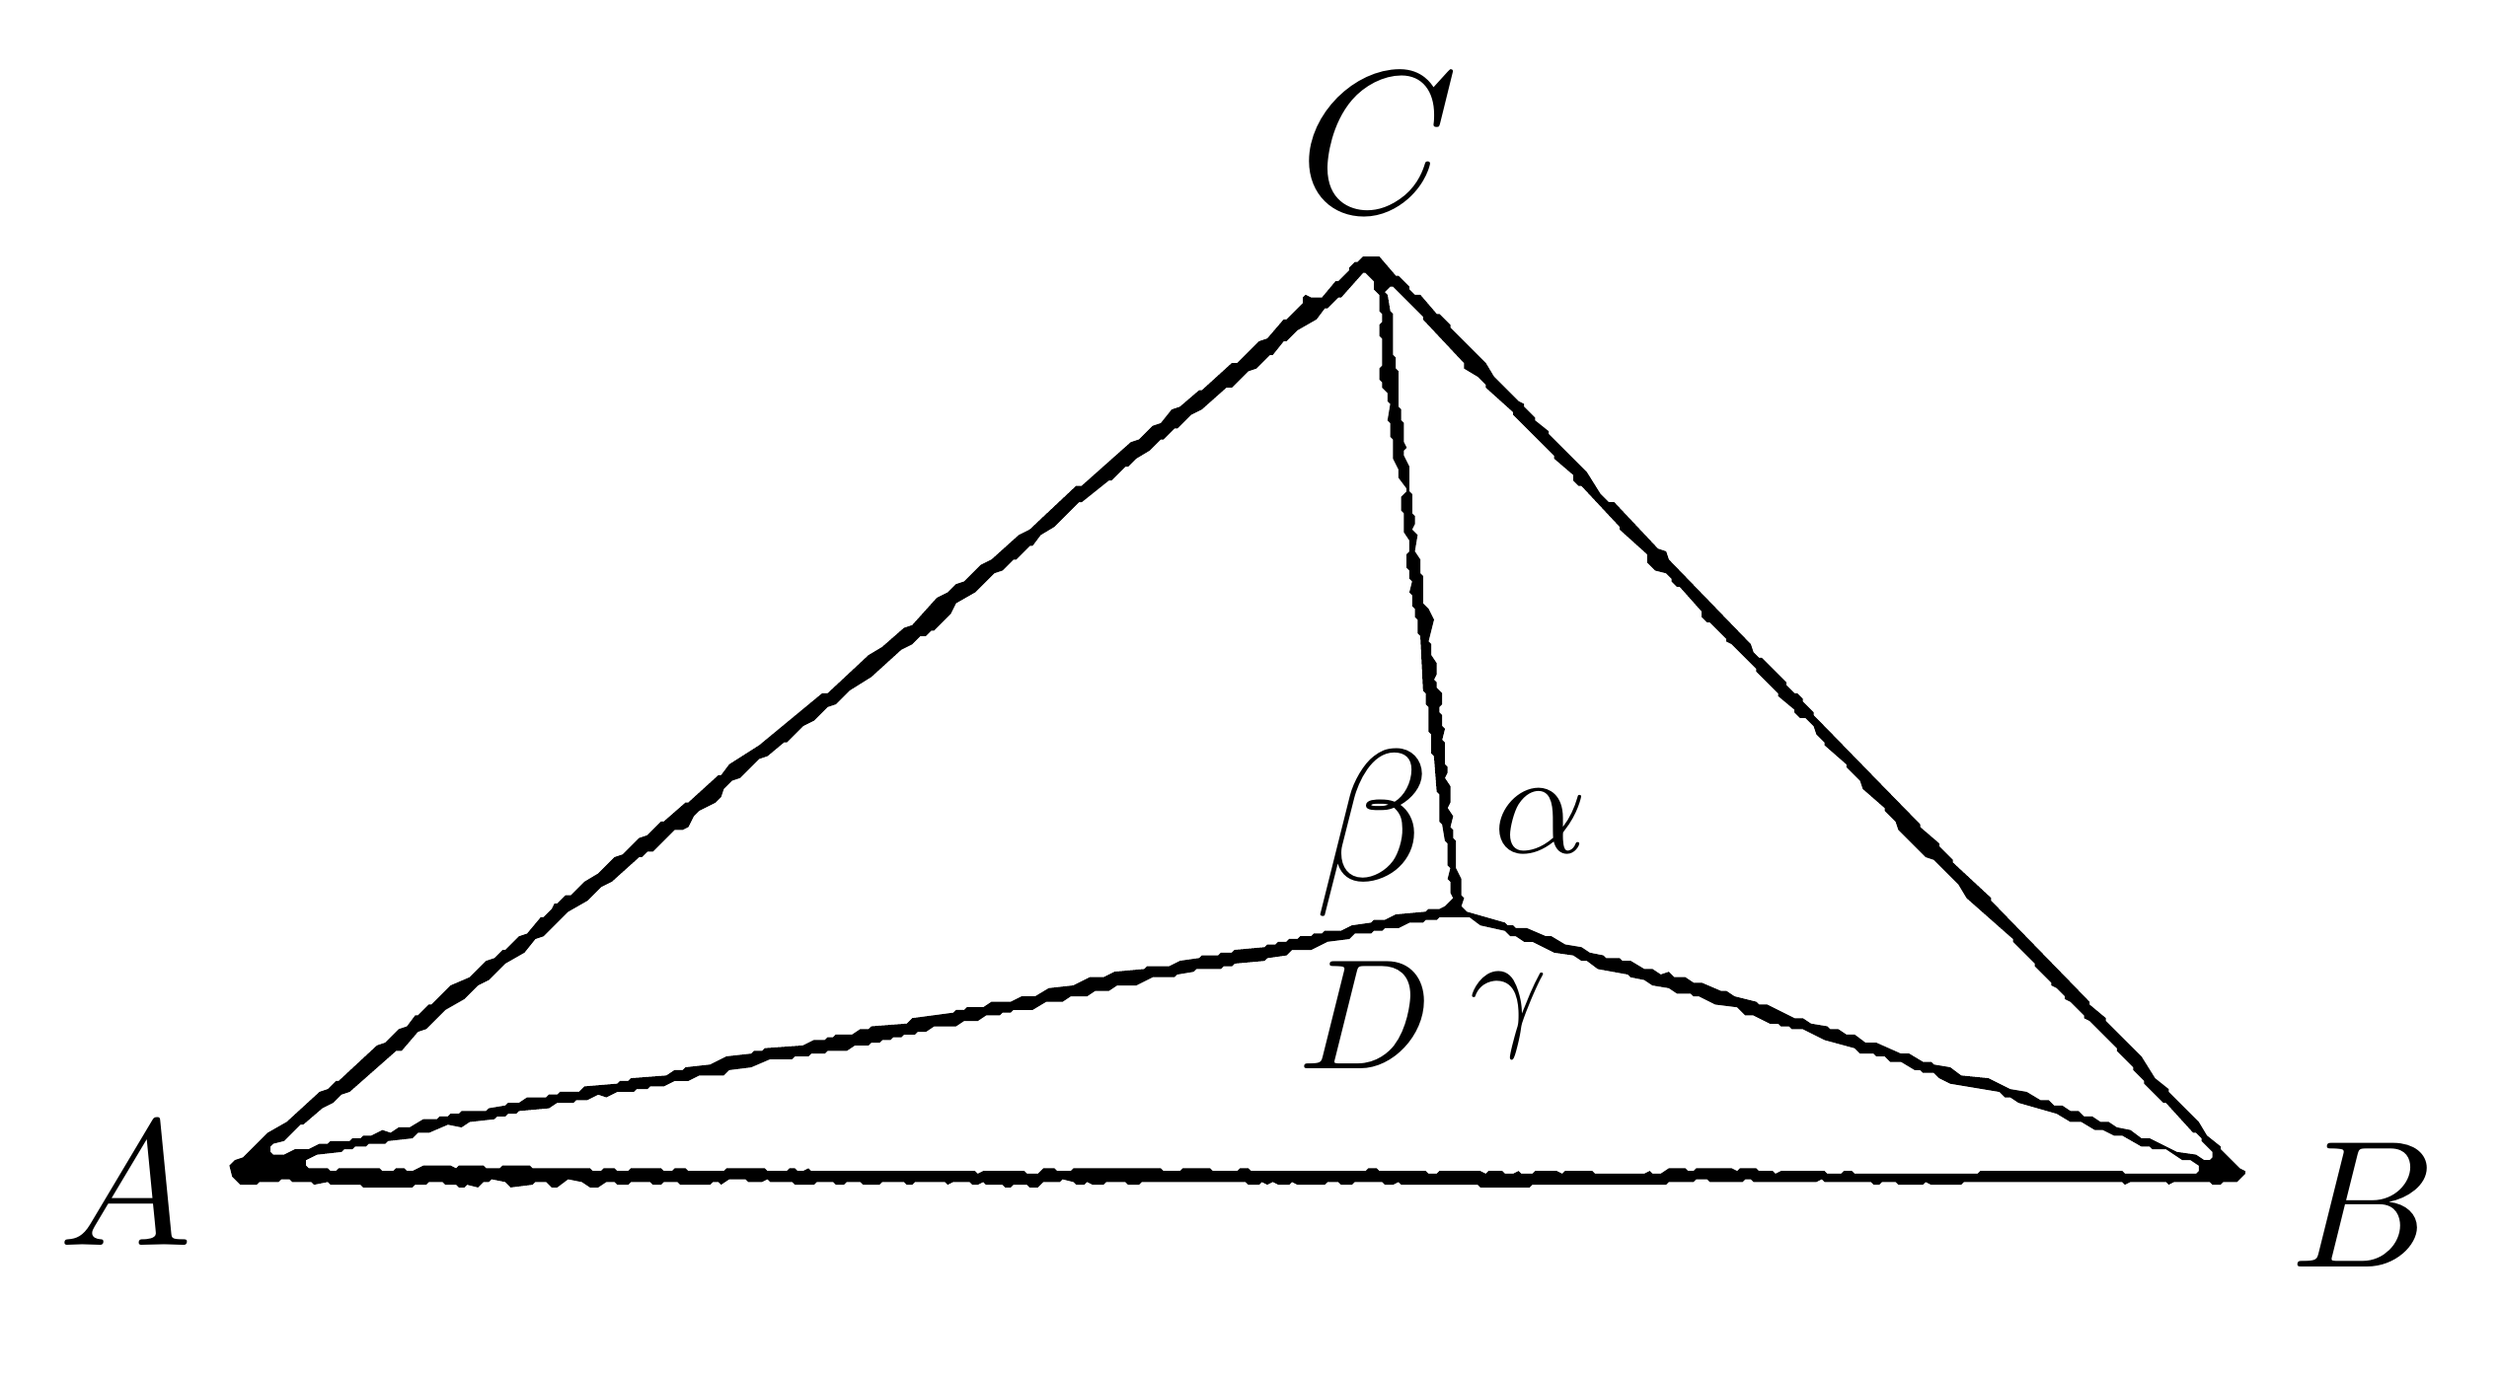
\begin{tikzpicture}[x=1pt,y=-1pt]
\path[use as bounding box] (0,0) rectangle (895,483);
\path[fill=black,draw=none,even odd rule]
(812,419) -- (810,418) -- (803,411) -- (803,410) -- (798,406) -- (795,401) -- (784,390) -- (784,389) -- (779,385) -- (774,377) -- (761,364) -- (761,363) -- (755,358) -- (755,357) -- (719,320) -- (719,319) -- (705,306) -- (705,305) -- (700,300) -- (700,299) -- (693,293) -- (693,292) -- (654,252) -- (654,251) -- (650,247) -- (650,246) -- (648,244) -- (647,244) -- (644,241) -- (644,240) -- (635,231) -- (634,231) -- (632,229) -- (631,226) -- (601,195) -- (600,192) -- (597,191) -- (581,174) -- (579,174) -- (576,171) -- (571,163) -- (557,149) -- (557,148) -- (552,144) -- (552,143) -- (548,139) -- (548,138) -- (546,137) -- (537,128) -- (534,123) -- (521,110) -- (521,109) -- (517,105) -- (516,105) -- (510,98) -- (508,98) -- (506,96) -- (506,95) -- (502,91) -- (501,91) -- (495,84) -- (489,84) -- (487,86) -- (486,86) -- (484,88) -- (484,89) -- (480,93) -- (479,93) -- (474,99) -- (470,99) -- (468,98) -- (467,99) -- (467,101) -- (461,107) -- (460,107) -- (454,114) -- (451,115) -- (443,123) -- (441,123) -- (430,133) -- (429,133) -- (422,139) -- (419,140) -- (415,145) -- (412,146) -- (407,151) -- (404,152) -- (386,168) -- (384,168) -- (367,184) -- (363,186) -- (353,195) -- (349,197) -- (343,203) -- (340,204) -- (337,207) -- (333,209) -- (324,219) -- (321,220) -- (313,227) -- (308,230) -- (293,244) -- (291,244) -- (268,263) -- (257,270) -- (254,274) -- (253,274) -- (242,284) -- (241,284) -- (233,291) -- (232,291) -- (227,296) -- (224,297) -- (218,303) -- (215,304) -- (209,310) -- (204,313) -- (199,318) -- (197,318) -- (194,321) -- (193,321) -- (192,323) -- (189,326) -- (188,326) -- (183,332) -- (180,333) -- (175,338) -- (174,338) -- (171,341) -- (168,342) -- (162,348) -- (155,351) -- (148,358) -- (147,358) -- (143,362) -- (142,362) -- (139,366) -- (136,367) -- (131,372) -- (128,373) -- (114,386) -- (113,386) -- (110,389) -- (107,390) -- (95,401) -- (88,405) -- (79,414) -- (76,415) -- (74,417) -- (75,421) -- (78,424) -- (84,424) -- (85,423) -- (92,423) -- (93,422) -- (96,422) -- (97,423) -- (104,423) -- (105,424) -- (110,423) -- (111,424) -- (122,424) -- (123,425) -- (141,425) -- (142,424) -- (146,424) -- (147,423) -- (152,423) -- (153,424) -- (157,424) -- (158,425) -- (160,425) -- (161,424) -- (165,425) -- (167,423) -- (169,423) -- (170,422) -- (175,423) -- (177,425) -- (185,424) -- (186,423) -- (190,423) -- (192,425) -- (194,425) -- (198,422) -- (203,423) -- (206,425) -- (209,425) -- (212,423) -- (215,423) -- (216,424) -- (220,424) -- (221,423) -- (228,423) -- (229,424) -- (232,424) -- (233,423) -- (238,423) -- (239,424) -- (250,424) -- (251,423) -- (253,423) -- (254,424) -- (257,422) -- (263,422) -- (264,423) -- (269,423) -- (271,422) -- (272,423) -- (280,423) -- (281,424) -- (288,424) -- (289,423) -- (295,423) -- (296,424) -- (299,424) -- (300,423) -- (305,423) -- (306,424) -- (312,424) -- (313,423) -- (321,423) -- (322,424) -- (324,424) -- (325,423) -- (336,423) -- (337,424) -- (339,423) -- (345,423) -- (346,424) -- (348,424) -- (350,423) -- (351,424) -- (357,424) -- (358,425) -- (360,425) -- (361,424) -- (366,424) -- (367,425) -- (370,425) -- (372,423) -- (378,423) -- (379,422) -- (383,423) -- (384,424) -- (387,424) -- (388,423) -- (390,424) -- (394,424) -- (395,423) -- (402,423) -- (403,424) -- (407,424) -- (408,423) -- (446,423) -- (447,424) -- (451,424) -- (452,423) -- (454,424) -- (456,423) -- (458,424) -- (462,424) -- (463,423) -- (465,424) -- (475,424) -- (476,423) -- (480,423) -- (481,424) -- (485,424) -- (486,423) -- (496,423) -- (497,424) -- (500,424) -- (502,423) -- (503,424) -- (531,424) -- (532,425) -- (550,425) -- (551,424) -- (600,424) -- (601,423) -- (610,423) -- (611,422) -- (615,422) -- (616,423) -- (628,423) -- (629,422) -- (631,422) -- (632,423) -- (655,423) -- (657,422) -- (658,423) -- (675,423) -- (676,424) -- (678,424) -- (679,423) -- (684,423) -- (685,424) -- (694,424) -- (695,423) -- (697,424) -- (708,424) -- (709,423) -- (767,423) -- (768,424) -- (770,423) -- (783,423) -- (784,424) -- (786,423) -- (799,423) -- (800,424) -- (803,424) -- (804,423) -- (809,423) -- (812,420) -- cycle
(795,419) -- (794,420) -- (768,420) -- (767,419) -- (715,419) -- (714,420) -- (669,420) -- (668,419) -- (665,419) -- (664,420) -- (659,420) -- (658,419) -- (642,419) -- (640,420) -- (639,419) -- (634,419) -- (633,418) -- (627,418) -- (626,419) -- (624,418) -- (611,418) -- (610,419) -- (608,419) -- (607,418) -- (601,418) -- (598,420) -- (595,420) -- (594,419) -- (592,420) -- (574,420) -- (573,419) -- (563,419) -- (562,420) -- (560,419) -- (552,419) -- (551,420) -- (547,420) -- (546,419) -- (544,420) -- (541,420) -- (540,419) -- (535,419) -- (534,420) -- (532,419) -- (517,419) -- (516,420) -- (513,420) -- (512,419) -- (495,419) -- (494,418) -- (491,418) -- (490,419) -- (448,419) -- (447,418) -- (444,418) -- (443,419) -- (434,419) -- (433,418) -- (423,418) -- (422,419) -- (416,419) -- (415,418) -- (383,418) -- (382,419) -- (377,419) -- (376,418) -- (372,418) -- (370,420) -- (366,420) -- (365,419) -- (350,419) -- (348,420) -- (347,419) -- (287,419) -- (286,418) -- (284,419) -- (282,419) -- (281,418) -- (279,418) -- (278,419) -- (271,419) -- (270,418) -- (256,418) -- (255,419) -- (242,419) -- (241,418) -- (237,418) -- (236,419) -- (233,419) -- (232,418) -- (221,418) -- (220,419) -- (216,419) -- (215,418) -- (211,418) -- (210,419) -- (207,419) -- (206,418) -- (185,418) -- (184,417) -- (174,417) -- (173,418) -- (168,418) -- (167,417) -- (158,417) -- (157,418) -- (155,417) -- (145,417) -- (141,419) -- (139,419) -- (138,418) -- (135,418) -- (134,419) -- (130,419) -- (129,418) -- (114,418) -- (113,419) -- (111,419) -- (110,418) -- (103,418) -- (102,417) -- (102,415) -- (106,413) -- (115,412) -- (116,411) -- (119,411) -- (120,410) -- (124,410) -- (125,409) -- (131,409) -- (132,408) -- (141,407) -- (143,405) -- (147,405) -- (154,402) -- (159,403) -- (162,401) -- (171,400) -- (172,399) -- (175,399) -- (176,398) -- (179,398) -- (180,397) -- (191,396) -- (194,394) -- (200,394) -- (201,393) -- (205,393) -- (209,391) -- (212,392) -- (216,390) -- (222,390) -- (223,389) -- (227,389) -- (228,388) -- (233,388) -- (237,386) -- (242,386) -- (246,384) -- (255,384) -- (257,382) -- (265,381) -- (272,378) -- (280,378) -- (281,377) -- (286,377) -- (287,376) -- (292,376) -- (293,375) -- (300,375) -- (303,373) -- (308,373) -- (309,372) -- (312,372) -- (313,371) -- (316,371) -- (317,370) -- (320,370) -- (321,369) -- (325,369) -- (326,368) -- (329,368) -- (332,366) -- (340,366) -- (343,364) -- (348,364) -- (351,362) -- (356,362) -- (357,361) -- (360,361) -- (361,360) -- (368,360) -- (373,357) -- (379,357) -- (382,355) -- (388,355) -- (391,353) -- (396,353) -- (399,351) -- (406,351) -- (412,348) -- (420,348) -- (421,347) -- (427,346) -- (428,345) -- (437,345) -- (438,344) -- (441,344) -- (442,343) -- (453,342) -- (454,341) -- (461,340) -- (463,338) -- (470,338) -- (476,335) -- (484,334) -- (486,332) -- (492,332) -- (493,331) -- (496,331) -- (497,330) -- (502,330) -- (506,328) -- (511,328) -- (512,327) -- (516,327) -- (517,326) -- (528,326) -- (532,329) -- (541,331) -- (543,333) -- (545,333) -- (548,335) -- (551,335) -- (559,339) -- (566,340) -- (569,342) -- (571,342) -- (575,345) -- (586,347) -- (587,348) -- (592,349) -- (595,351) -- (601,352) -- (604,354) -- (609,354) -- (610,355) -- (612,355) -- (618,358) -- (626,359) -- (629,362) -- (632,362) -- (638,365) -- (641,365) -- (642,366) -- (645,366) -- (646,367) -- (650,367) -- (658,371) -- (669,374) -- (671,376) -- (676,376) -- (677,377) -- (680,377) -- (682,379) -- (686,379) -- (691,382) -- (693,382) -- (694,383) -- (698,383) -- (700,385) -- (704,387) -- (722,390) -- (724,392) -- (726,392) -- (729,394) -- (743,398) -- (748,401) -- (752,401) -- (757,404) -- (760,404) -- (764,406) -- (767,406) -- (774,410) -- (777,410) -- (778,411) -- (783,411) -- (789,415) -- (792,415) -- (795,417) -- cycle
(499,95) -- (500,95) -- (511,106) -- (511,107) -- (526,123) -- (526,125) -- (531,128) -- (534,131) -- (534,132) -- (544,141) -- (544,142) -- (559,157) -- (559,158) -- (566,164) -- (566,166) -- (568,168) -- (569,168) -- (583,183) -- (583,184) -- (593,193) -- (593,196) -- (596,199) -- (600,200) -- (602,202) -- (602,203) -- (604,205) -- (605,205) -- (613,214) -- (613,216) -- (615,218) -- (616,218) -- (622,224) -- (622,225) -- (624,226) -- (633,235) -- (633,236) -- (641,244) -- (641,245) -- (647,250) -- (647,251) -- (649,253) -- (651,253) -- (654,256) -- (655,259) -- (658,262) -- (658,263) -- (666,270) -- (666,271) -- (671,276) -- (672,279) -- (680,286) -- (680,287) -- (684,291) -- (685,294) -- (695,304) -- (698,305) -- (707,314) -- (710,319) -- (727,334) -- (727,335) -- (735,343) -- (735,344) -- (741,350) -- (741,351) -- (743,352) -- (746,355) -- (746,356) -- (748,357) -- (753,362) -- (753,363) -- (755,364) -- (765,374) -- (765,375) -- (771,381) -- (771,382) -- (775,386) -- (775,387) -- (782,394) -- (783,394) -- (793,405) -- (794,405) -- (796,407) -- (796,408) -- (800,412) -- (800,414) -- (799,415) -- (797,415) -- (794,413) -- (787,412) -- (777,407) -- (774,407) -- (770,404) -- (765,403) -- (762,401) -- (759,401) -- (756,399) -- (753,399) -- (751,397) -- (748,397) -- (745,395) -- (742,395) -- (740,393) -- (737,393) -- (732,390) -- (726,389) -- (718,385) -- (708,384) -- (704,381) -- (698,380) -- (697,379) -- (694,379) -- (689,376) -- (686,376) -- (677,372) -- (673,372) -- (669,369) -- (666,369) -- (663,367) -- (660,367) -- (659,366) -- (653,365) -- (650,363) -- (647,363) -- (637,358) -- (634,358) -- (633,357) -- (625,355) -- (622,353) -- (620,353) -- (613,350) -- (610,350) -- (607,348) -- (603,348) -- (601,346) -- (598,347) -- (595,345) -- (592,345) -- (587,342) -- (584,342) -- (583,341) -- (578,341) -- (577,340) -- (572,339) -- (569,337) -- (563,336) -- (558,333) -- (556,333) -- (549,330) -- (545,330) -- (544,329) -- (542,329) -- (541,328) -- (527,324) -- (525,322) -- (526,319) -- (525,318) -- (525,312) -- (523,308) -- (523,298) -- (522,297) -- (522,294) -- (521,293) -- (522,289) -- (520,286) -- (521,284) -- (521,278) -- (519,275) -- (520,273) -- (520,271) -- (519,270) -- (519,262) -- (518,261) -- (519,257) -- (518,256) -- (518,252) -- (517,251) -- (517,249) -- (518,248) -- (518,244) -- (516,242) -- (516,240) -- (515,239) -- (516,237) -- (516,233) -- (514,230) -- (514,226) -- (513,225) -- (515,217) -- (513,213) -- (511,211) -- (511,201) -- (510,200) -- (510,195) -- (508,192) -- (509,186) -- (507,184) -- (508,182) -- (508,179) -- (507,178) -- (507,171) -- (506,170) -- (506,161) -- (504,157) -- (504,155) -- (505,154) -- (504,152) -- (504,145) -- (503,144) -- (503,140) -- (502,139) -- (502,126) -- (501,125) -- (501,121) -- (500,120) -- (500,105) -- (499,104) -- (498,98) -- (497,97) -- cycle
(493,93) -- (493,96) -- (495,98) -- (495,104) -- (496,105) -- (496,108) -- (495,109) -- (495,113) -- (496,114) -- (496,124) -- (495,125) -- (495,129) -- (496,130) -- (496,132) -- (498,134) -- (498,137) -- (499,138) -- (498,144) -- (499,145) -- (499,150) -- (500,151) -- (500,158) -- (502,162) -- (502,165) -- (505,169) -- (505,170) -- (503,172) -- (503,177) -- (504,178) -- (504,185) -- (506,188) -- (506,192) -- (505,193) -- (505,198) -- (506,199) -- (506,202) -- (507,203) -- (506,207) -- (507,208) -- (507,212) -- (508,213) -- (508,216) -- (509,217) -- (509,222) -- (510,223) -- (511,243) -- (512,244) -- (512,248) -- (513,249) -- (513,258) -- (514,259) -- (514,266) -- (515,267) -- (516,280) -- (517,281) -- (517,291) -- (518,292) -- (519,298) -- (520,299) -- (520,307) -- (521,308) -- (520,312) -- (521,313) -- (521,317) -- (522,319) -- (519,322) -- (517,323) -- (513,323) -- (512,324) -- (501,325) -- (497,327) -- (493,327) -- (492,328) -- (485,329) -- (481,331) -- (475,331) -- (474,332) -- (471,332) -- (470,333) -- (466,333) -- (465,334) -- (462,334) -- (461,335) -- (458,335) -- (457,336) -- (454,336) -- (453,337) -- (442,338) -- (441,339) -- (437,339) -- (436,340) -- (430,340) -- (429,341) -- (422,342) -- (418,344) -- (410,344) -- (409,345) -- (398,346) -- (394,348) -- (389,348) -- (383,351) -- (374,352) -- (369,355) -- (364,355) -- (360,357) -- (353,357) -- (350,359) -- (344,359) -- (343,360) -- (340,360) -- (339,361) -- (324,363) -- (322,365) -- (309,366) -- (308,367) -- (305,367) -- (302,369) -- (296,369) -- (295,370) -- (293,370) -- (292,371) -- (288,371) -- (284,373) -- (270,374) -- (269,375) -- (266,375) -- (265,376) -- (256,377) -- (250,380) -- (241,381) -- (240,382) -- (237,382) -- (234,384) -- (221,385) -- (220,386) -- (217,386) -- (216,387) -- (204,388) -- (202,390) -- (195,390) -- (194,391) -- (191,391) -- (190,392) -- (183,392) -- (180,394) -- (176,394) -- (175,395) -- (169,396) -- (168,397) -- (159,397) -- (158,398) -- (155,398) -- (154,399) -- (151,399) -- (150,400) -- (145,400) -- (140,403) -- (136,403) -- (133,405) -- (130,404) -- (126,406) -- (123,406) -- (122,407) -- (119,407) -- (118,408) -- (111,408) -- (110,409) -- (107,409) -- (103,411) -- (98,411) -- (94,413) -- (90,413) -- (89,412) -- (89,410) -- (90,409) -- (94,408) -- (100,402) -- (101,402) -- (108,396) -- (112,394) -- (115,391) -- (118,390) -- (135,375) -- (137,375) -- (143,368) -- (146,367) -- (153,360) -- (160,356) -- (165,351) -- (169,349) -- (175,343) -- (182,339) -- (186,334) -- (189,333) -- (198,324) -- (205,320) -- (210,315) -- (214,313) -- (224,304) -- (225,304) -- (227,302) -- (229,302) -- (237,294) -- (240,294) -- (242,293) -- (244,289) -- (246,287) -- (252,284) -- (254,282) -- (255,279) -- (258,276) -- (261,275) -- (268,268) -- (271,267) -- (277,262) -- (278,262) -- (284,256) -- (288,254) -- (293,249) -- (296,248) -- (301,243) -- (309,238) -- (320,228) -- (324,226) -- (327,223) -- (329,223) -- (331,221) -- (332,221) -- (338,215) -- (340,211) -- (347,207) -- (354,200) -- (357,199) -- (361,195) -- (362,195) -- (367,190) -- (368,190) -- (371,186) -- (376,183) -- (385,174) -- (386,174) -- (396,166) -- (397,166) -- (402,161) -- (403,161) -- (406,158) -- (411,155) -- (415,151) -- (416,151) -- (420,147) -- (421,147) -- (426,142) -- (430,140) -- (439,132) -- (441,132) -- (447,126) -- (450,125) -- (455,120) -- (456,120) -- (460,115) -- (461,115) -- (465,111) -- (472,107) -- (475,103) -- (476,103) -- (480,99) -- (481,99) -- (489,90) -- (490,90) -- cycle;
\node[inner sep=0pt,font=\fontsize{10}{10}\selectfont] at (495.0,42.5) {\scalebox{7.425}{$C$}};
\node[inner sep=0pt,font=\fontsize{10}{10}\selectfont] at (36.0,424.0) {\scalebox{6.534}{$A$}};
\node[inner sep=0pt,font=\fontsize{10}{10}\selectfont] at (855.5,431.5) {\scalebox{6.633}{$B$}};
\node[inner sep=0pt,font=\fontsize{10}{10}\selectfont] at (490.0,362.0) {\scalebox{5.742}{$D$}};
\node[inner sep=0pt,font=\fontsize{10}{10}\selectfont] at (554.0,291.0) {\scalebox{5.346}{$\alpha$}};
\node[inner sep=0pt,font=\fontsize{10}{10}\selectfont] at (492.5,295.5) {\scalebox{6.831}{$\beta$}};
\node[inner sep=0pt,font=\fontsize{10}{10}\selectfont] at (542.5,362.0) {\scalebox{4.95}{$\gamma$}};
\end{tikzpicture}%
}
\end{center}

Für den zweiten Fall ist der Ausdruck ein ganz ähnlicher, den ich Kürze halber übergehe.

Um noch einmal auf das \textls[120]{Criterium} zurückzukommen, bemerke ich,
